\section{Evaluation} \label{sec:evaluation}

\begin{figure*}[t]
\centering
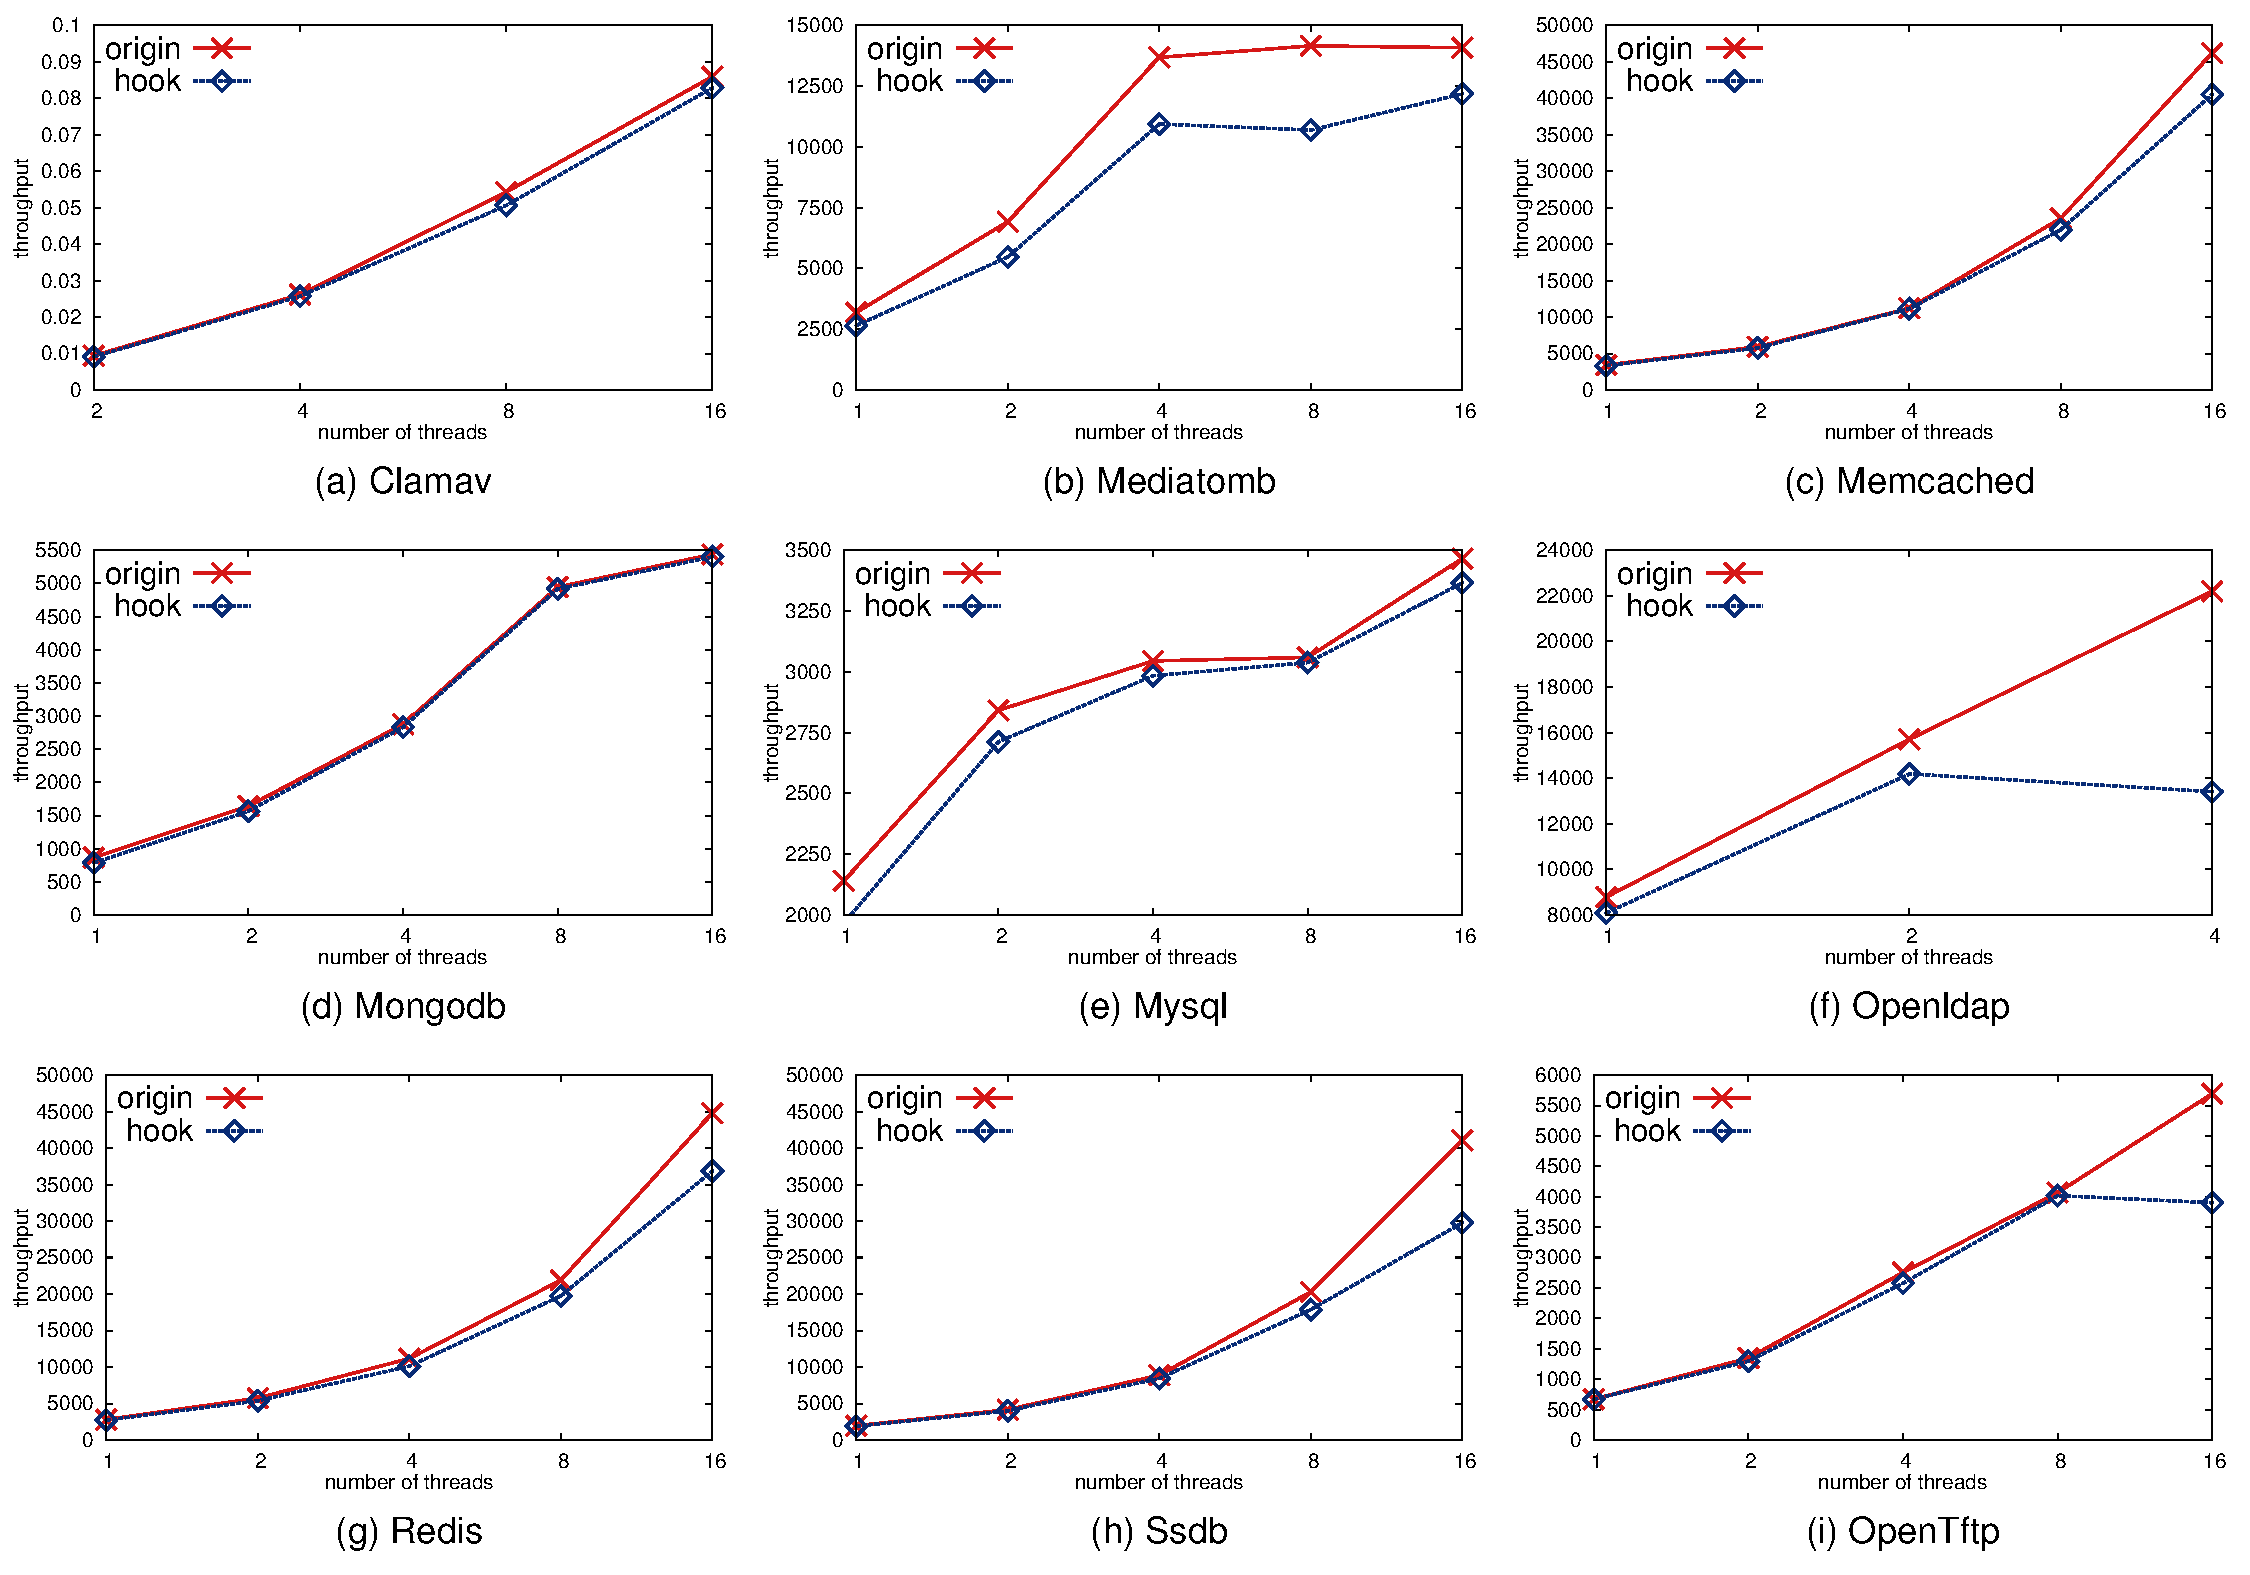
\includegraphics[width=0.9\textwidth]{figures/throughput}
\vspace{-.20in}
\caption{\small {\em \xxx throughput compared to the unreplicated 
execution.}}
\label{fig:tput}
\end{figure*}

\begin{figure*}[t]
\centering
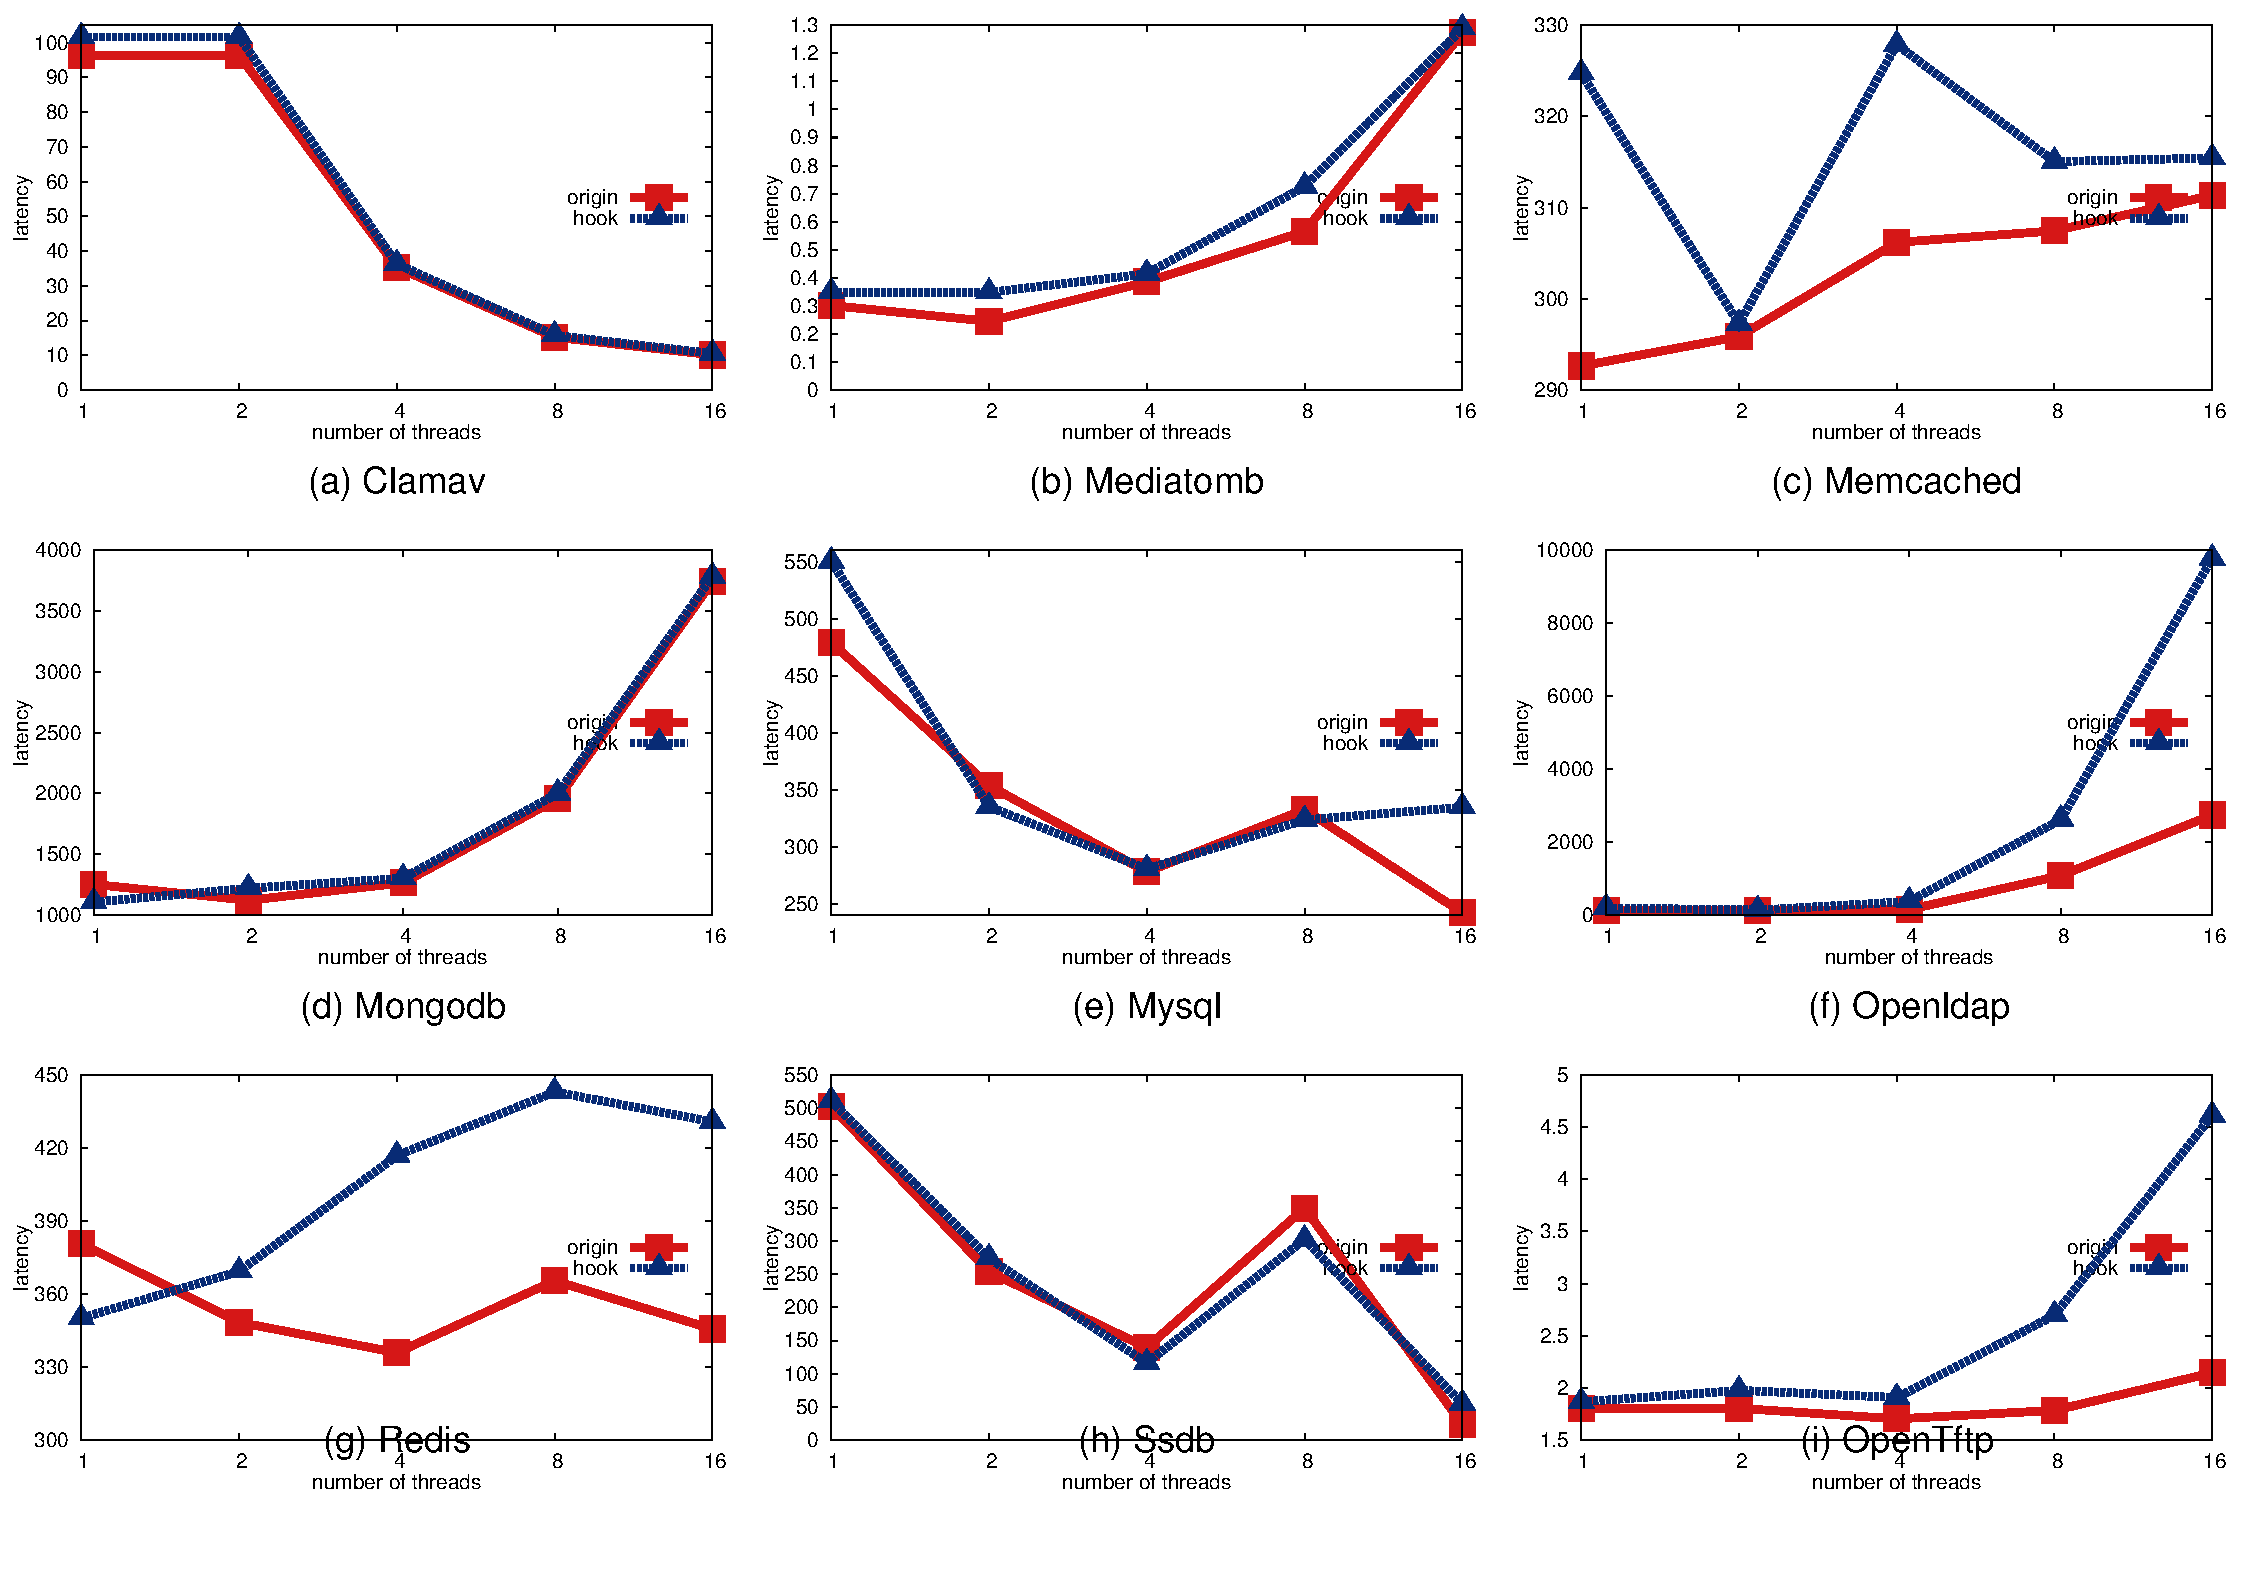
\includegraphics[width=0.9\textwidth]{figures/latency}
\vspace{-.20in}
\caption{\small {\em \xxx response time (latency) compared to the unreplicated 
execution.}}
\label{fig:latency}
\end{figure*}

Our evaluation used three Dell R430 servers as SMR replicas. Each server having 
Linux 3.16.0, 2.6 GHz Intel Xeon CPU with 24 hyper-threading cores, 32GB 
memory, and 1T SSD. Each machine has a Mellanox ConnectX-3 Pro Dual Port 40 Gbps 
NIC. These NICs are connected using the Infiniband RDMA architecture through a 
Dell S6000 high-performance switch with 32 40Gpbs ports. The \v{ping} latency 
between every two replicas are 84 \us. This latency is achieved through IPoIB 
(IP over Infiniband), the optimal latency for a client to communicate with a 
server through traditional TCP/IP between replica machines.

To mitigate network latency of public network, all client benchmarks were ran 
in a Dell R320 server (the client machine), with Linux 3.16.0, 2.2GHz Intel 
Xeon with 12 hyper-threading cores, 32GB memory, and 160G SSD. This server 
connects with the replica machines with 1Gbps bandwidth LAN. The average 
\v{ping} latency between the client machine and a replica machine is 301 \us. A 
larger network latency (\eg, sending client requests from WAN) will further 
mask \xxx's overhead.

We evaluated \xxx on \nprog widely used or studied server programs, including 
\nkvprog key-value stores \redis, \memcached, \ssdb, \mongodb; \mysql, a SQL 
server; \clamav, a anti-virus server that scans files and delete malicious ones; 
\mediatomb, a multimedia storage server that stores and transcodes video and 
audeo files; \openldap, an LDAP server; \calvin, a widely studied transactional 
database system that leverages \zookeeper as its SMR service. All these programs 
are multithreaded except \redis (but it can still serve requests concurrently 
using Libevent). These servers all update or store important data and files, 
thus the high fault-tolerance of SMR is especially attractive to these programs.

\begin{table}[b]
\footnotesize
\centering
\vspace{-.05in}
\begin{tabular}{lrr}
{\bf Program} & {\bf Benchmark} & {\bf Workload/input description}\\
\hline\\[-2.3ex]
\clamav & clamscan  & Files in \v{/lib} from same replica \\
\mediatomb & ApacheBench  & Transcode video files in parallel\\
\memcached & mcperf  & 50\% set and 50\% put operations\\
\mongodb & YCSB  & Workload C\\
\mysql & Sysbench  & Concurrent SQL transactions\\
\openldap & Self  & TBD\\
\redis & Self  & 50\% set and 50\% put operations\\
\ssdb & Self  & 50\% set and 50\% put operations\\
\calvin & Self  & Concurrent SQL transactions\\
\end{tabular}
\vspace{-.05in}
\caption{{\em Benchmarks and workloads.} ``Self" in the Benchmark column means 
we used a server program's own performance benchmark program.} 
\label{tab:benchmarks}
\end{table}

% Benchmarks table.
Table~\ref{tab:benchmarks} introduces the benchmarks and workloads we used. To 
evaluate \xxx's practicality, we used the server developers' own performance 
benchmarks or popular third-party. For benchmark workload settings, we used the 
benchmarks' default workloads whenever available. We spawned 
up to 16 concurrent connections which made these servers approach peak 
throughput, and then we measured both response time (latency) and throughput. We 
also measured \xxx's bare consensus latency. All evaluation results were done 
with a replica group size of three except the scalability evaluation 
(\S\ref{sec:scalability}). Each performance data point in the evaluation is 
taken from the mean value of 10 repeated executions.

% evaluation metric. client benchmarks all run in LAN, average latency
The rest of this section focuses on these questions:

\begin{tightenum}

\item[\S\ref{sec:ease-of-use}:] How easy is it to run general server programs 
in \xxx?

\item[\S\ref{sec:overhead}:] What is \xxx's performance compared to the 
unreplicated executions? What is \xxx's consensus latency on input coordination 
and output checking?

\item[\S\ref{sec:scalability}:] How scalable is \xxx on different replica group 
sizes?

\item[\S\ref{sec:compare}:] What is \xxx's performance compared to existing 
SMR systems?

\item[\S\ref{sec:robust}:] How fast can \xxx recover replicas from output 
divergence?

% \item[\S\ref{sec:race}:] If some \xxx users care about data races much, how 
% does \xxx tolerate the slowdown of data race detector by deploying it on a 
% replica?

% \item[\S\ref{sec:lesson}:] What practical lessons have we learnt during the 
% case study on these server programs with \xxx?

\end{tightenum}

\subsection{Ease of Use} \label{sec:ease-of-use}

\xxx is able to run all \nprog evaluated programs without modifying them except 
for \calvin. \calvin integrates its client program and server program within the 
same process and uses local memory to send transactions from the client to 
server. To make \calvin's client and server communicate with POSIX sockets so 
that \xxx can intercept client inputs, we wrote a \nlinescalvin patch for 
\calvin.

\subsection{Performance Overhead} \label{sec:overhead}

Figure~\ref{fig:tput} shows \xxx's throughput and Figure~\ref{fig:latency} 
response time. We varied the number of concurrent client connections for each 
server program by from one to 16 threads or until they reached peak performance. 
For \calvin, we only collected the 8-thread result because \calvin used this 
constant thread count to serve client requests. Overall, compared to these 
server programs' unreplicated executions, \xxx merely incurred a mean 
througput degrade by \tputoverhead (note that in Figure~\ref{fig:tput}, the 
Y-axises of most programs start from a large number). \xxx's mean overhead on 
response time was merely \latencyoverhead.

As the number of threads increases, all programs' unreplicated executions 
got a perforamnce improvement except \memcached. A prior 
evaluation~\cite{rex:eurosys14} also observed a similar \memcached low 
scalability. \xxx scaled almost as well as the unreplicated executions.
% a \latencyoverhead overhead compared to the unreplicated 
% executions.

\xxx achieves such low overhead in both throughput and response time due to two 
reasons. First, for each \recv call in a server program, \xxx's input 
coordination protocol only contains two one-sided RDMA writes and two SSD writes 
between each leader and backup. Second, \xxx's output checking protocol, which 
is based on the input coordination protocol, invokes extremely occasionally, 
once for every \thashcomp output hash generations (\S\ref{sec:output-workflow}).

\begin{table}[b]
\footnotesize
\centering
\vspace{-.05in}
\begin{tabular}{lrrrr}
{\bf Program} & {\bf \# Calls} & {\bf Input} & {\bf SSD time} 
& {\bf Quorum time}\\
\hline\\[-2.3ex]
% Heming: normalized clamav to 10K req.
\clamav & 30,000  & 42.0 & 4.9 \us & 7.2 \us\\
% TBD: normalize mediatomb to 10K req.
\mediatomb & 30,000  & 140.0 & 4.4 \us & 6.9 \us\\
\memcached & 10,016  & 38.0 & 4.6 \us & 6.3 \us\\
\mongodb & 10,376  & 492.4 & 14.9 \us & 16.4 \us\\
\mysql & 10,009  & 26.0 & 5.0 \us & 8.4 \us\\
% TBD: normalize ldap to 10K req.
\openldap & 10,016  & 27.3 & 6.4 \us & 12.0 \us\\
\redis & 10,016  & 107.0 & 3.7 \us & 6.3 \us\\
% TBD: normalize ssdb to 10K req.
\ssdb & 10,016  & 47.0 & 3.7 \us & 10.9 \us\\
\calvin & 10,002  & 93.0 & 2.5 \us  & 9.9 \us\\
\end{tabular}
\vspace{-.05in}
\caption{{\em Leader's input consensus events per 10K requests.} 
The ``\# Calls" column means the number of socket calls that went through \xxx 
input concensus; ``Input" means average bytes of a server's inputs received in 
these calls; ``SSD time" means the average time spent on storing these calls to 
stable storage; and ``Quorum time" means the average time spent on waiting 
quorum for these calls.} 
\label{tab:consensus-latency}
\end{table}

% Figure~\ref{fig:latency} shows \xxx's latency.
% % Bare consensus latency, micro events.

To deeply understand \xxx's performance overhread, we collected the number of 
socket call events and consensus durations in the leader replica. 
Table~\ref{tab:consensus-latency} shows these statistics for every 10K requests. 
For each socket call, \xxx's leader invokes a consensus, which includes an SSD 
write phase (the ``SSD time" column in Table~\ref{tab:consensus-latency}) and a 
quorum waiting phase (the ``quorum time" column). The quorum waiting phase 
implies replicas' performance because each replica stores the proposed socket 
call into SSD and then sends a consensus reply by doing an RDMA write to the 
leader. 

By summing these two time columns, overall, a \xxx input consensus took only 
9.9 \us (\redis) to 39.6 \us (\mongodb). This consensus latency mainly depends 
on the ``Input" column: the average number of data bytes received in socket 
calls (\eg, \mongodb has the largest received bytes). \xxx's small consensus 
latency makes \xxx achieve reasonable throughputs in Figure~\ref{fig:tput} and 
response times Figure~\ref{fig:latency}. This small latency suggests that \xxx 
may still achieve acceptable overhead on some programs even if clients are 
deployed within the same datacenter network, although \xxx's default deployment 
model is running server replicas in a datacenter and clients in LAN or WAN.

\subsection{Comparison with Traditional SMR systems} \label{sec:compare}

We compared \xxx with \calvin's SMR system because \calvin's inpur consensus 
uses \zookeeper, one of the most widely used coordination service built on 
TCP/IP. To conduct a fair comparison, both \xxx and \calvin SMR, we ran 
\calvin's own transactional database as the server program, and we compared 
throughputs and the consensus latency. \xxx achieved 17.6K transactions/s with a 
12.5 \us consensus latency. \calvin achieved 19.9K transactions/s with a 511.9 
\us consensus latency. The throughput in \calvin was 13.1\% higher than that in 
\xxx because \calvin puts transactions in a batch with a 10 \ms timeout and then 
it invokes \zookeeper for consensus on this batch. Batching helps \calvin 
ahieves good throughput. \xxx currently has not incorporated a batching 
techinque because its latency is already reasonably fast (\S\ref{sec:overhead}).

Notably, \xxx's consensus latency was 40.1X faster than \zookeeper's mainly due 
to \xxx's RDMA-accelerated consensus protocol. A prior SMR
evaluation~\cite{dare:hpdc15} also reports a similar 320 \us \zookeeper 
consensus latency as we got. This \xxx-\calvin comparison suggests that \calvin 
will be better if clients prefer high throughput, and \xxx will be better if 
clients demand short latency.

% Comparison with Crane. Run Crane. TBD


\subsection{Scalability on Replica Group Size} \label{sec:scalability}

% TBD: rerun \redis micro events; it is too small, so we can not use it here.

Because we had only three RDMA-enable machines in the evaluation time, we 
picked \redis as the testing program and ran five \xxx instances on three 
machines: one machine held the leader instance, and each of the other two 
machines held two backups.

Given the same \redis workload, \xxx had a 17.9K throughput and 10.0 \us 
consensus latency. Compared to the three-node setting, 18.0K throughput and 9.9 
\us consensus latency, \xxx is quite scalable. For seven nodes XXX TBD. We plan 
to buy more server machines for a larger scale of scalability evaluation.

% It 
% would be interesting to see whether \xxx's scalability on replica group size is 
% bounded by the outbound RDMA writes of RDMA NICs.



% Comparison with DARE. Three to five nodes.

\subsection{Recovering from Output Divergence} \label{sec:robust}

Once an output divergence is detected, \xxx will roll bacak the divergent 
replica, including leader and backups. For all the \nprog programs, our output 
checking protocol found these servers produced identical results except \clamav 
and \ssdb.

\clamav's divergent output is caused by its special threading model: 
unlike the other evaluated programs which use one thread to server one client 
connection, \clamav uses multiple worker threads to serve a client request 
(\eg, scanning a directory path recursively). \xxx's worker threads 
concurrently contend for a global mutex lock and then append the scanned 
files into the output buffer for the client, causing a nondeterministic order 
of scanned files among all replicas. We manually compared \clamav's output 
across replicas, and we found the files were indeed the same except their order.

We ran \ssdb on the same workload as in \S\ref{sec:overhead} and triggered a 
previous unkown concurrency bug in the QPUSH operations. This concurrency bug 
was triggered by concurrent client connections to push elements to a queue in 
\ssdb. In our evaluation, this bug was first triggered in a backup machine and 
caused a divergent output hash. the hashes of the other two replicas were 
still the same. \xxx's leader detected this divergence; it sent a 
rollback request to the divergent replica's guard, which took 1.2 \ms; 
the guard killed the \ssdb server and restored it from a prior 
checkpoint with 0.913 \ms, and the recovered replica reconnected to the other 
replicas and started to server requests in 0.09 \ms. Each process and file 
system checkpoint operation for \ssdb took 954 \ms.

This minor divergence suggests that we hitted a bug, for two 
reasons. First, \xxx has enfored strongly consistent inputs across replicas, if 
only replicas diverge, this divergence must be caused by the server program 
itself, not different inputs. Second, only one replica diverged, this suggests 
that the output does not contain randome values (\eg, physical times, or the 
\clamav case), otherwise all replicas should diverged.

We then carefully looked into the \ssdb source code and identified the bug. It 
was caused by incorrect synchronization to a global queue in \ssdb. We have 
reported this bug to the \ssdb developers with a suggested bug fixing 
patch~\cite{ssdb:bug}. Although \xxx does not intend to find bugs, this 
promising finding reflects that \xxx could be extended as an advanced testing 
tool: its fast, general SMR service lets it easily support general program, and 
its consistently enforce inputs and efficient output checking makes the minor 
replica output divergence a strong software bug indicator.
% Confidence. strongly consistent inputs.

% 
% \subsection{Sensitivity of Parameters} \label{sec:sensitivity}

% Change output comparison periods. 1, 100, 1000, 10000. 1000 is the smallest 
% number that starts to have negligible overhead. Run only with the server with 
% largest recv() data size.

% Twait

% Tcomphash
 
% \subsection{Read-only Optimization} \label{sec:read-opt}

% % 